\chapter{Modellauswertung}\label{chap:metrics}
\section{Metriken}
Der mAP (mean Average Precision) ist eine Metrik, mit der die Leistung von Modellen zur Objekterkennung bewertet werden kann. Der mAP-Wert wird für verschiedene IoU-Schwellenwerte berechnet. mAP@0.5:0.95 deckt einen großen Bereich von IoU-Schwellen ab. Der mAP@0.5 gibt an, wie gut das Modell Objekte bei einer IoU-Schwelle von 0.5 erkennt. mAP@0.75 gibt die Leistung bei einer höheren IoU-Schwelle von 0.75 an. Diese Metriken bewerten die Erkennungs- und Lokalisierungsgenauigkeit des Modells bei verschiedenen Überlappungsschwellen (IoU-Werten). Sie dienen dem Vergleich und der Bewertung der Modelle. Ein höherer mAP-Wert bedeutet eine bessere Leistung bei der Erkennung von Objekten mit dieser spezifischen Überlappungsschwelle.

Die beiden Tabellen \ref{tab:metricVal} und \ref{tab:metricTest} liefern eine Bewertung der Leistung von YOLOX und YOLOv8 anhand verschiedener Metriken. Die erste Tabelle basiert auf dem Validierungsdatensatz, der während des Trainings zur Validierung verwendet wurde, während die zweite Tabelle den unabhängigen Testdatensatz zeigt, der zu Beginn der Arbeit abgespalten wurde.

Bei dem Vergleich der Gesamtleistung des Modells (Klasse: all) ist YOLOv8 in allen Werten um 2 \% besser als YOLOX. Die relativ ähnlichen Werte sind wahrscheinlich auf die ähnliche Architektur der beiden Modelle zurückzuführen. Die Erhöhung der Leistung ist auf die Verwendung des DFL zurückzuführen.

\begin{table}[!ht]
	\centering
	\renewcommand{\arraystretch}{1.1} % Anpassung der Zellhöhe
	\begin{tabular}{|l|>{\arraybackslash}p{1.5cm}|>{\arraybackslash}p{1.5cm}|>{\arraybackslash}p{1.5cm}|>{\arraybackslash}p{1.5cm}|>{\arraybackslash}p{1.5cm}|>{\arraybackslash}p{1.5cm}|}
		\hline
		\textbf{} & \multicolumn{2}{c|}{\textbf{mAP@0.5:0.95}} & \multicolumn{2}{c|}{\textbf{mAP@0.5}} & \multicolumn{2}{c|}{\textbf{mAP@0.75}} \\ \cline{2-7}
		\textbf{} & YOLOX & YOLOv8 & YOLOX & YOLOv8 & YOLOX & YOLOv8 \\ \hline
		\textbf{all} & 0.484 & \textbf{0.501} & 0.776 & \textbf{0.793} & 0.508  & \textbf{0.528} \\ \hline
		\textbf{car} & 0.567 & \textbf{0.607} & 0.845 &\textbf{ 0.873} & 0.633 & \textbf{0.684} \\ 
		\textbf{pedestrian} & \textbf{0.348} & 0.342 & \textbf{0.690} & 0.67 & \textbf{0.307} & 0.297 \\
		\textbf{trafficLight} & 0.473 & \textbf{0.499} & 0.784 & \textbf{0.831} & 0.465 & \textbf{0.501} \\
		\textbf{truck} & 0.628 & \textbf{0.646} & 0.864 & \textbf{0.877} & 0.726 & \textbf{0.743} \\
		\textbf{biker} & 0.403 & \textbf{0.412} & 0.696 & \textbf{0.713} & 0.412 & \textbf{0.416} \\ \hline
	\end{tabular}
	\caption{Vergleich der mAP Werte für den Validierungsdatensatz. Quelle: Eigene Darstellung}
	\label{tab:metricVal}
\end{table}

\begin{table}[!ht]
	\centering
	\renewcommand{\arraystretch}{1.1} % Anpassung der Zellhöhe
	\begin{tabular}{|l|>{\arraybackslash}p{1.5cm}|>{\arraybackslash}p{1.5cm}|>{\arraybackslash}p{1.5cm}|>{\arraybackslash}p{1.5cm}|>{\arraybackslash}p{1.5cm}|>{\arraybackslash}p{1.5cm}|}
		\hline
		\textbf{} & \multicolumn{2}{c|}{\textbf{mAP@0.5:0.95}} & \multicolumn{2}{c|}{\textbf{mAP@0.5}} & \multicolumn{2}{c|}{\textbf{mAP@0.75}} \\ \cline{2-7}
		\textbf{} & YOLOX & YOLOv8 & YOLOX & YOLOv8 & YOLOX & YOLOv8 \\ \hline
		\textbf{all} & 0.484 & \textbf{0.498} & 0.776 & \textbf{0.794} & 0.508  & \textbf{0.523} \\ \hline
		\textbf{car} & 0.568 & \textbf{0.609} & 0.838 &\textbf{ 0.873} & 0.638 & \textbf{0.691} \\ 
		\textbf{pedestrian} & \textbf{0.365} & 0.36 & \textbf{0.724} & 0.703 & 0.304 & \textbf{0.316} \\
		\textbf{trafficLight} & 0.459 & \textbf{0.493} & 0.770 & \textbf{0.817} & 0.465 & \textbf{0.505} \\
		\textbf{truck} & 0.594 & \textbf{0.612} & 0.83 & \textbf{0.835} & 0.665 & \textbf{0.696} \\
		\textbf{biker} & \textbf{0.431} & 0.414 & 0.732 & \textbf{0.741} & \textbf{0.484} & 0.406 \\ \hline
	\end{tabular}
	\caption{Vergleich der mAP Werte für den Testdatensatz. Quelle: Eigene Darstellung}
	\label{tab:metricTest}
\end{table}



\section{Vorhersage}
In der Abbildung \ref{fig:predictionNetworks} ist auf der linken Seite die Ausgabe von YOLOX dargestellt und auf der rechten Seite die Ausgabe von YOLOv8. Beide Netzwerke sind mit dem gleichen Testdatensatz durchlaufen, um die Bounding Boxen auf den Bildern zu erzeugen.

\begin{figure}[htbp]
	\centering
	\begin{subfigure}[b]{0.35\textwidth}
		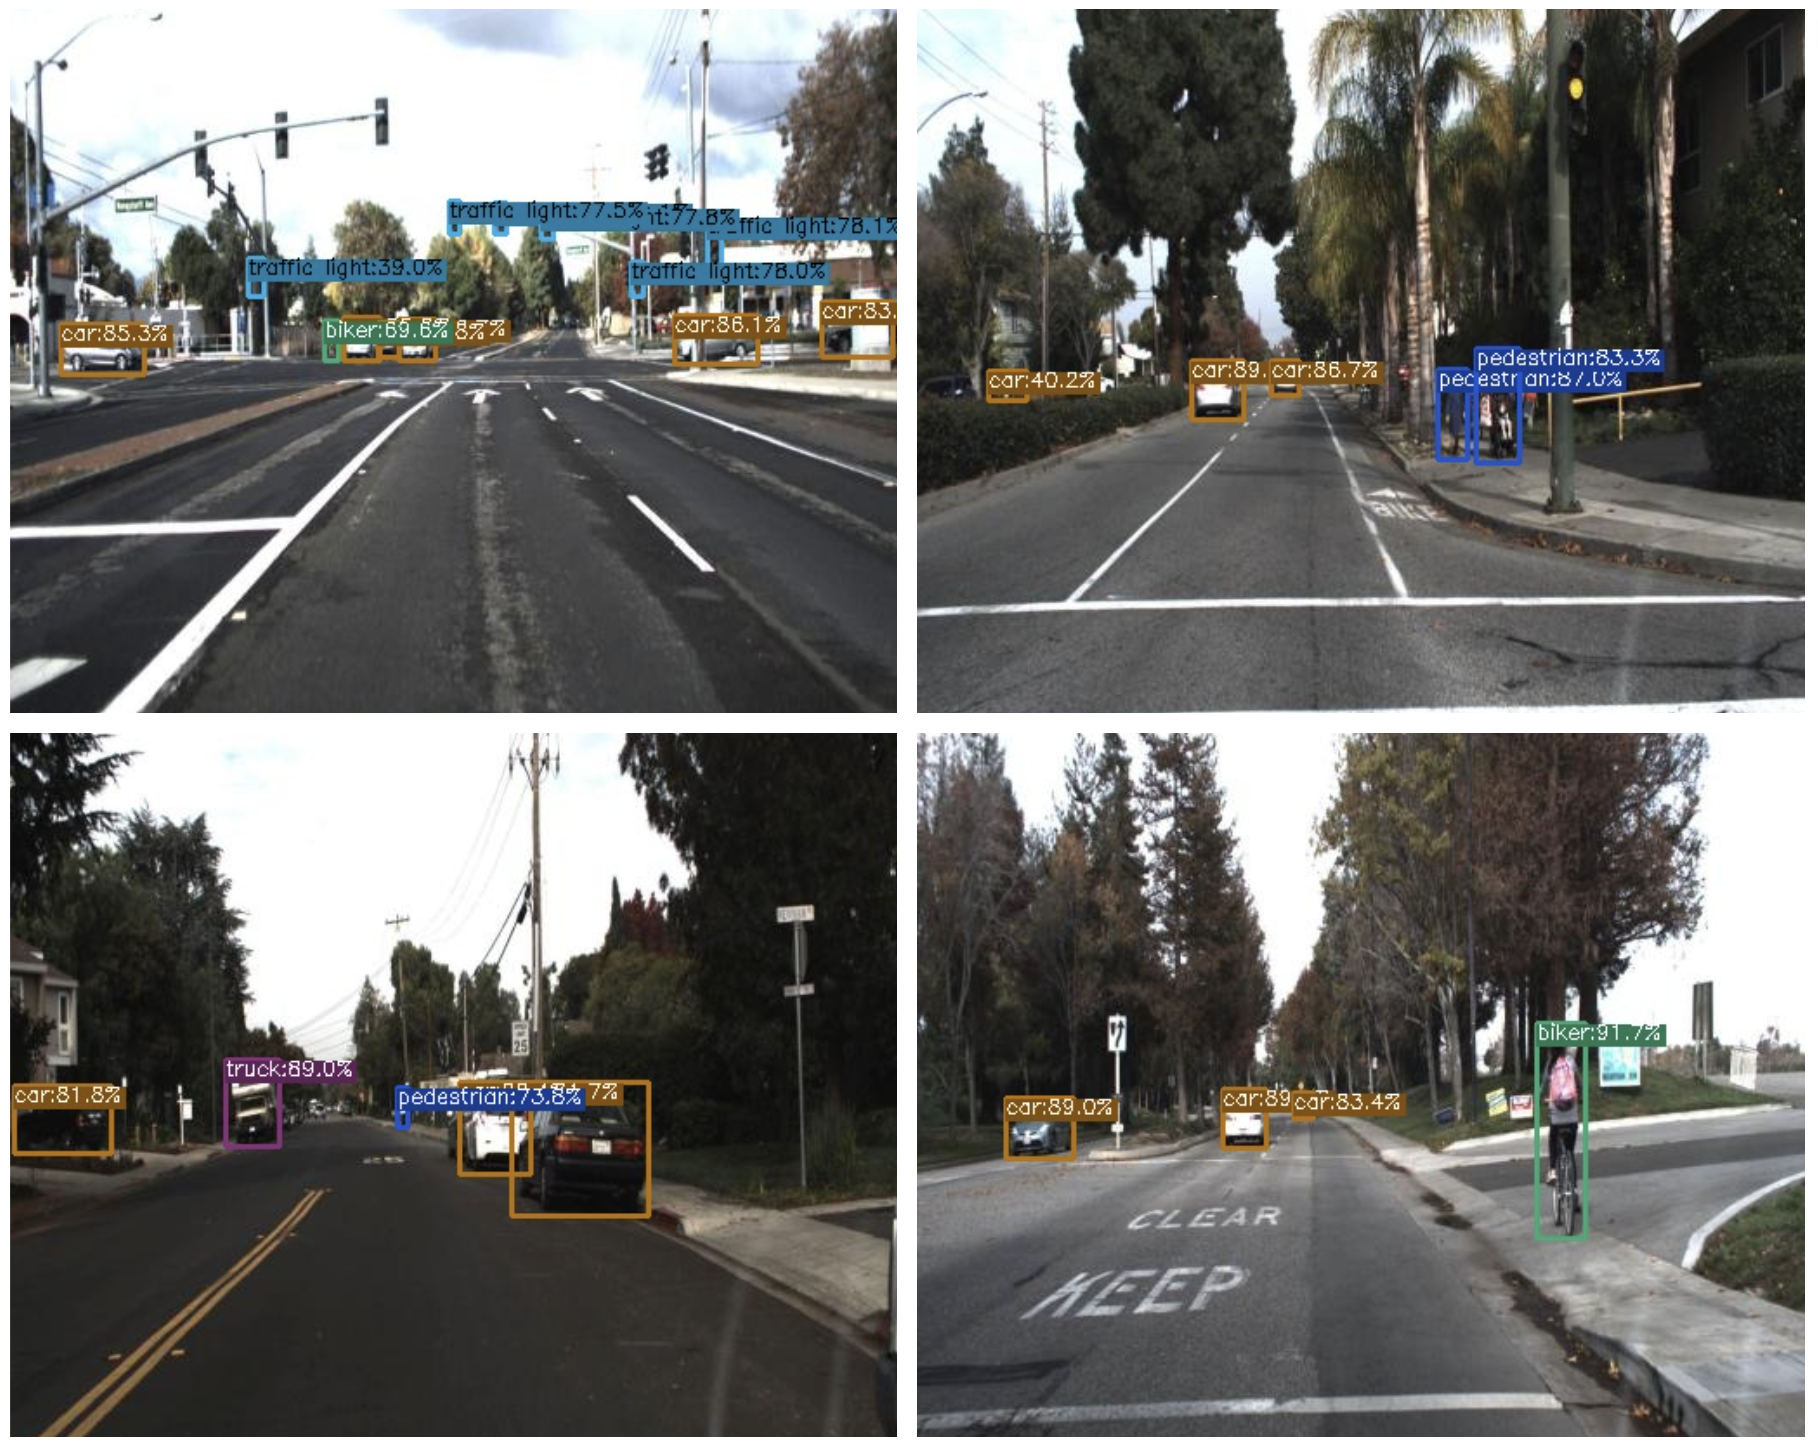
\includegraphics[width=\textwidth]{predictYOLOX.png}
	\end{subfigure}
	\hspace{0.1cm} % Anpassung des Abstands
	\begin{subfigure}[b]{0.35\textwidth}
		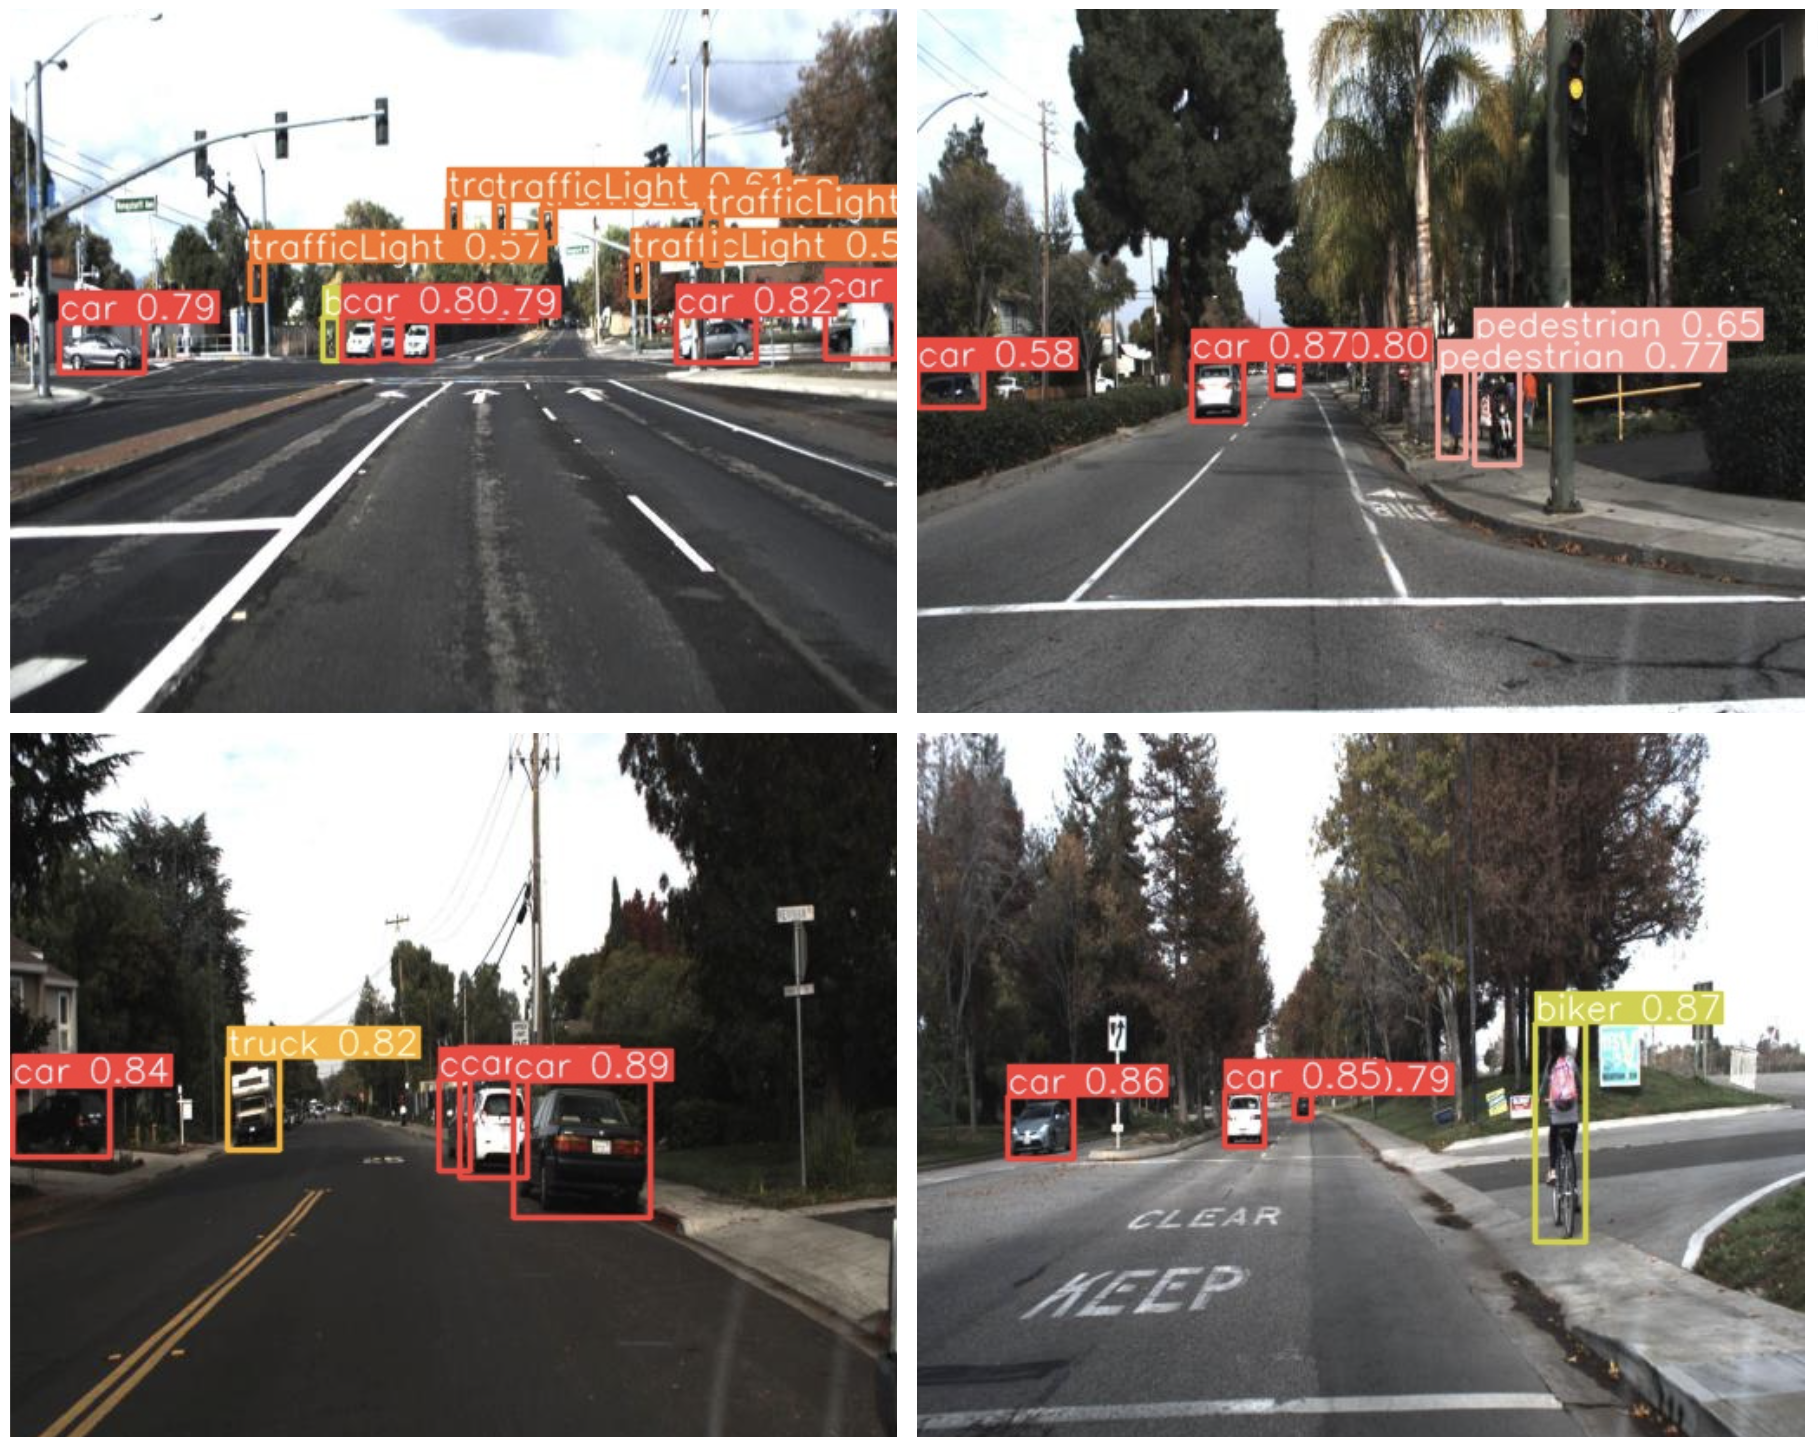
\includegraphics[width=\textwidth]{predictYOLOv8.png}
	\end{subfigure}
	\caption[Vorhersage der Netzwerke auf vier Beispielbildern aus dem Testdatensatz]{Vorhersage der Netzwerke auf vier Beispielbildern aus dem Testdatensatz (links: YOLOX, rechts: YOLOv8). Quelle: Eigene Aufnahme}
	\label{fig:predictionNetworks}
\end{figure}

